% Options for packages loaded elsewhere
\PassOptionsToPackage{unicode}{hyperref}
\PassOptionsToPackage{hyphens}{url}
\PassOptionsToPackage{dvipsnames,svgnames,x11names}{xcolor}
%
\documentclass[
  letterpaper,
  DIV=11,
  numbers=noendperiod]{scrartcl}

\usepackage{amsmath,amssymb}
\usepackage{lmodern}
\usepackage{iftex}
\ifPDFTeX
  \usepackage[T1]{fontenc}
  \usepackage[utf8]{inputenc}
  \usepackage{textcomp} % provide euro and other symbols
\else % if luatex or xetex
  \usepackage{unicode-math}
  \defaultfontfeatures{Scale=MatchLowercase}
  \defaultfontfeatures[\rmfamily]{Ligatures=TeX,Scale=1}
\fi
% Use upquote if available, for straight quotes in verbatim environments
\IfFileExists{upquote.sty}{\usepackage{upquote}}{}
\IfFileExists{microtype.sty}{% use microtype if available
  \usepackage[]{microtype}
  \UseMicrotypeSet[protrusion]{basicmath} % disable protrusion for tt fonts
}{}
\makeatletter
\@ifundefined{KOMAClassName}{% if non-KOMA class
  \IfFileExists{parskip.sty}{%
    \usepackage{parskip}
  }{% else
    \setlength{\parindent}{0pt}
    \setlength{\parskip}{6pt plus 2pt minus 1pt}}
}{% if KOMA class
  \KOMAoptions{parskip=half}}
\makeatother
\usepackage{xcolor}
\setlength{\emergencystretch}{3em} % prevent overfull lines
\setcounter{secnumdepth}{-\maxdimen} % remove section numbering
% Make \paragraph and \subparagraph free-standing
\ifx\paragraph\undefined\else
  \let\oldparagraph\paragraph
  \renewcommand{\paragraph}[1]{\oldparagraph{#1}\mbox{}}
\fi
\ifx\subparagraph\undefined\else
  \let\oldsubparagraph\subparagraph
  \renewcommand{\subparagraph}[1]{\oldsubparagraph{#1}\mbox{}}
\fi

\usepackage{color}
\usepackage{fancyvrb}
\newcommand{\VerbBar}{|}
\newcommand{\VERB}{\Verb[commandchars=\\\{\}]}
\DefineVerbatimEnvironment{Highlighting}{Verbatim}{commandchars=\\\{\}}
% Add ',fontsize=\small' for more characters per line
\usepackage{framed}
\definecolor{shadecolor}{RGB}{241,243,245}
\newenvironment{Shaded}{\begin{snugshade}}{\end{snugshade}}
\newcommand{\AlertTok}[1]{\textcolor[rgb]{0.68,0.00,0.00}{#1}}
\newcommand{\AnnotationTok}[1]{\textcolor[rgb]{0.37,0.37,0.37}{#1}}
\newcommand{\AttributeTok}[1]{\textcolor[rgb]{0.40,0.45,0.13}{#1}}
\newcommand{\BaseNTok}[1]{\textcolor[rgb]{0.68,0.00,0.00}{#1}}
\newcommand{\BuiltInTok}[1]{\textcolor[rgb]{0.00,0.23,0.31}{#1}}
\newcommand{\CharTok}[1]{\textcolor[rgb]{0.13,0.47,0.30}{#1}}
\newcommand{\CommentTok}[1]{\textcolor[rgb]{0.37,0.37,0.37}{#1}}
\newcommand{\CommentVarTok}[1]{\textcolor[rgb]{0.37,0.37,0.37}{\textit{#1}}}
\newcommand{\ConstantTok}[1]{\textcolor[rgb]{0.56,0.35,0.01}{#1}}
\newcommand{\ControlFlowTok}[1]{\textcolor[rgb]{0.00,0.23,0.31}{#1}}
\newcommand{\DataTypeTok}[1]{\textcolor[rgb]{0.68,0.00,0.00}{#1}}
\newcommand{\DecValTok}[1]{\textcolor[rgb]{0.68,0.00,0.00}{#1}}
\newcommand{\DocumentationTok}[1]{\textcolor[rgb]{0.37,0.37,0.37}{\textit{#1}}}
\newcommand{\ErrorTok}[1]{\textcolor[rgb]{0.68,0.00,0.00}{#1}}
\newcommand{\ExtensionTok}[1]{\textcolor[rgb]{0.00,0.23,0.31}{#1}}
\newcommand{\FloatTok}[1]{\textcolor[rgb]{0.68,0.00,0.00}{#1}}
\newcommand{\FunctionTok}[1]{\textcolor[rgb]{0.28,0.35,0.67}{#1}}
\newcommand{\ImportTok}[1]{\textcolor[rgb]{0.00,0.46,0.62}{#1}}
\newcommand{\InformationTok}[1]{\textcolor[rgb]{0.37,0.37,0.37}{#1}}
\newcommand{\KeywordTok}[1]{\textcolor[rgb]{0.00,0.23,0.31}{#1}}
\newcommand{\NormalTok}[1]{\textcolor[rgb]{0.00,0.23,0.31}{#1}}
\newcommand{\OperatorTok}[1]{\textcolor[rgb]{0.37,0.37,0.37}{#1}}
\newcommand{\OtherTok}[1]{\textcolor[rgb]{0.00,0.23,0.31}{#1}}
\newcommand{\PreprocessorTok}[1]{\textcolor[rgb]{0.68,0.00,0.00}{#1}}
\newcommand{\RegionMarkerTok}[1]{\textcolor[rgb]{0.00,0.23,0.31}{#1}}
\newcommand{\SpecialCharTok}[1]{\textcolor[rgb]{0.37,0.37,0.37}{#1}}
\newcommand{\SpecialStringTok}[1]{\textcolor[rgb]{0.13,0.47,0.30}{#1}}
\newcommand{\StringTok}[1]{\textcolor[rgb]{0.13,0.47,0.30}{#1}}
\newcommand{\VariableTok}[1]{\textcolor[rgb]{0.07,0.07,0.07}{#1}}
\newcommand{\VerbatimStringTok}[1]{\textcolor[rgb]{0.13,0.47,0.30}{#1}}
\newcommand{\WarningTok}[1]{\textcolor[rgb]{0.37,0.37,0.37}{\textit{#1}}}

\providecommand{\tightlist}{%
  \setlength{\itemsep}{0pt}\setlength{\parskip}{0pt}}\usepackage{longtable,booktabs,array}
\usepackage{calc} % for calculating minipage widths
% Correct order of tables after \paragraph or \subparagraph
\usepackage{etoolbox}
\makeatletter
\patchcmd\longtable{\par}{\if@noskipsec\mbox{}\fi\par}{}{}
\makeatother
% Allow footnotes in longtable head/foot
\IfFileExists{footnotehyper.sty}{\usepackage{footnotehyper}}{\usepackage{footnote}}
\makesavenoteenv{longtable}
\usepackage{graphicx}
\makeatletter
\def\maxwidth{\ifdim\Gin@nat@width>\linewidth\linewidth\else\Gin@nat@width\fi}
\def\maxheight{\ifdim\Gin@nat@height>\textheight\textheight\else\Gin@nat@height\fi}
\makeatother
% Scale images if necessary, so that they will not overflow the page
% margins by default, and it is still possible to overwrite the defaults
% using explicit options in \includegraphics[width, height, ...]{}
\setkeys{Gin}{width=\maxwidth,height=\maxheight,keepaspectratio}
% Set default figure placement to htbp
\makeatletter
\def\fps@figure{htbp}
\makeatother

\usepackage{booktabs}
\usepackage{longtable}
\usepackage{array}
\usepackage{multirow}
\usepackage{wrapfig}
\usepackage{float}
\usepackage{colortbl}
\usepackage{pdflscape}
\usepackage{tabu}
\usepackage{threeparttable}
\usepackage{threeparttablex}
\usepackage[normalem]{ulem}
\usepackage{makecell}
\usepackage{xcolor}
\KOMAoption{captions}{tableheading}
\makeatletter
\makeatother
\makeatletter
\makeatother
\makeatletter
\@ifpackageloaded{caption}{}{\usepackage{caption}}
\AtBeginDocument{%
\ifdefined\contentsname
  \renewcommand*\contentsname{Table of contents}
\else
  \newcommand\contentsname{Table of contents}
\fi
\ifdefined\listfigurename
  \renewcommand*\listfigurename{List of Figures}
\else
  \newcommand\listfigurename{List of Figures}
\fi
\ifdefined\listtablename
  \renewcommand*\listtablename{List of Tables}
\else
  \newcommand\listtablename{List of Tables}
\fi
\ifdefined\figurename
  \renewcommand*\figurename{Figure}
\else
  \newcommand\figurename{Figure}
\fi
\ifdefined\tablename
  \renewcommand*\tablename{Table}
\else
  \newcommand\tablename{Table}
\fi
}
\@ifpackageloaded{float}{}{\usepackage{float}}
\floatstyle{ruled}
\@ifundefined{c@chapter}{\newfloat{codelisting}{h}{lop}}{\newfloat{codelisting}{h}{lop}[chapter]}
\floatname{codelisting}{Listing}
\newcommand*\listoflistings{\listof{codelisting}{List of Listings}}
\makeatother
\makeatletter
\@ifpackageloaded{caption}{}{\usepackage{caption}}
\@ifpackageloaded{subcaption}{}{\usepackage{subcaption}}
\makeatother
\makeatletter
\@ifpackageloaded{tcolorbox}{}{\usepackage[many]{tcolorbox}}
\makeatother
\makeatletter
\@ifundefined{shadecolor}{\definecolor{shadecolor}{named}{true}}
\makeatother
\makeatletter
\makeatother
\ifLuaTeX
  \usepackage{selnolig}  % disable illegal ligatures
\fi
\IfFileExists{bookmark.sty}{\usepackage{bookmark}}{\usepackage{hyperref}}
\IfFileExists{xurl.sty}{\usepackage{xurl}}{} % add URL line breaks if available
\urlstyle{same} % disable monospaced font for URLs
\hypersetup{
  pdftitle={Add the Time-Varying Variable into Markov Model},
  pdfauthor={Astrid Yu, Ashley Leech},
  colorlinks=true,
  linkcolor={blue},
  filecolor={Maroon},
  citecolor={Blue},
  urlcolor={Blue},
  pdfcreator={LaTeX via pandoc}}

\title{Add the Time-Varying Variable into Markov Model}
\author{Astrid Yu, Ashley Leech}
\date{2023-03-22}

\begin{document}
\maketitle
\ifdefined\Shaded\renewenvironment{Shaded}{\begin{tcolorbox}[boxrule=0pt, frame hidden, colback={shadecolor}, breakable, enhanced]}{\end{tcolorbox}}\fi

\renewcommand*\contentsname{Table of contents}
{
\hypersetup{linkcolor=}
\setcounter{tocdepth}{3}
\tableofcontents
}
Based on the last tutorial of Markov Model in R, we will add background
mortality using a cause-deleted life table.

\begin{Shaded}
\begin{Highlighting}[]
\FunctionTok{library}\NormalTok{(knitr)}
\CommentTok{\# knit(\textquotesingle{}MarkovDA.qmd\textquotesingle{}, tangle=TRUE)}
\CommentTok{\# source(\textquotesingle{}MarkovDA.R\textquotesingle{})}
\FunctionTok{source}\NormalTok{(}\FunctionTok{purl}\NormalTok{(}\StringTok{"MarkovDA.qmd"}\NormalTok{, }\AttributeTok{output =} \FunctionTok{tempfile}\NormalTok{()))}
\FunctionTok{options}\NormalTok{(}\StringTok{"scipen"}\OtherTok{=}\DecValTok{1000}\NormalTok{, }\StringTok{"digits"}\OtherTok{=}\DecValTok{2}\NormalTok{)}
\end{Highlighting}
\end{Shaded}

\hypertarget{dive-into-life-table}{%
\section{Dive into Life Table}\label{dive-into-life-table}}

\hypertarget{where-to-get-the-us-life-table}{%
\subsection{Where to get the US life
table}\label{where-to-get-the-us-life-table}}

\url{https://www.cdc.gov/nchs/products/life_tables.htm} {[}CDC
website{]}

We are using United States Life Tables(2020) -- remember to distinguish
the life tables for the male and the female.

Male:
\url{https://ftp.cdc.gov/pub/Health_Statistics/NCHS/Publications/NVSR/71-01/Table02.xlsx}

Female:
\url{https://ftp.cdc.gov/pub/Health_Statistics/NCHS/Publications/NVSR/71-01/Table03.xlsx}

\begin{longtable}[]{@{}ll@{}}
\toprule()
Name & Description \\
\midrule()
\endhead
qx & Probability of dying between ages x and x + 1 \\
lx & Number surviving to age x \\
dx & Number dying between ages x and x + 1 \\
Lx & Person-years lived between ages x and x + 1 \\
Tx & Total number of person-years lived above age x \\
ex & Expectation of life at age x \\
\bottomrule()
\end{longtable}

\begin{Shaded}
\begin{Highlighting}[]
\NormalTok{input\_file }\OtherTok{=} \FunctionTok{normalizePath}\NormalTok{(}\FunctionTok{here}\NormalTok{(}\StringTok{"exercise/markov\_exercise\_phd.xlsx"}\NormalTok{))}
\NormalTok{life\_table\_raw }\OtherTok{=}\NormalTok{ readxl}\SpecialCharTok{::}\FunctionTok{read\_xlsx}\NormalTok{(input\_file,}\AttributeTok{sheet=}\StringTok{"Life Table {-} Male"}\NormalTok{,}\AttributeTok{col\_types =}\StringTok{"numeric"}\NormalTok{)[}\SpecialCharTok{{-}}\DecValTok{1}\NormalTok{,]}
\FunctionTok{names}\NormalTok{(life\_table\_raw) }\OtherTok{=} \FunctionTok{c}\NormalTok{(}\StringTok{"Age"}\NormalTok{, }\StringTok{"qx"}\NormalTok{, }\StringTok{"lx"}\NormalTok{, }\StringTok{"dx"}\NormalTok{, }\StringTok{"Lx"}\NormalTok{, }\StringTok{"Tx"}\NormalTok{, }\StringTok{"ex"}\NormalTok{)}
\end{Highlighting}
\end{Shaded}

\hypertarget{where-to-get-the-specific-cause-death}{%
\subsection{Where to get the specific-cause
death}\label{where-to-get-the-specific-cause-death}}

Here we set all our patients are initially 45-yr men with the prostate
cancer.

\url{https://vizhub.healthdata.org/gbd-results/}{[}GBD query tool{]}

GBD results provide the \% of deaths due to a specific cause by age
(every 5 years) and sex groups.

Using filters like:

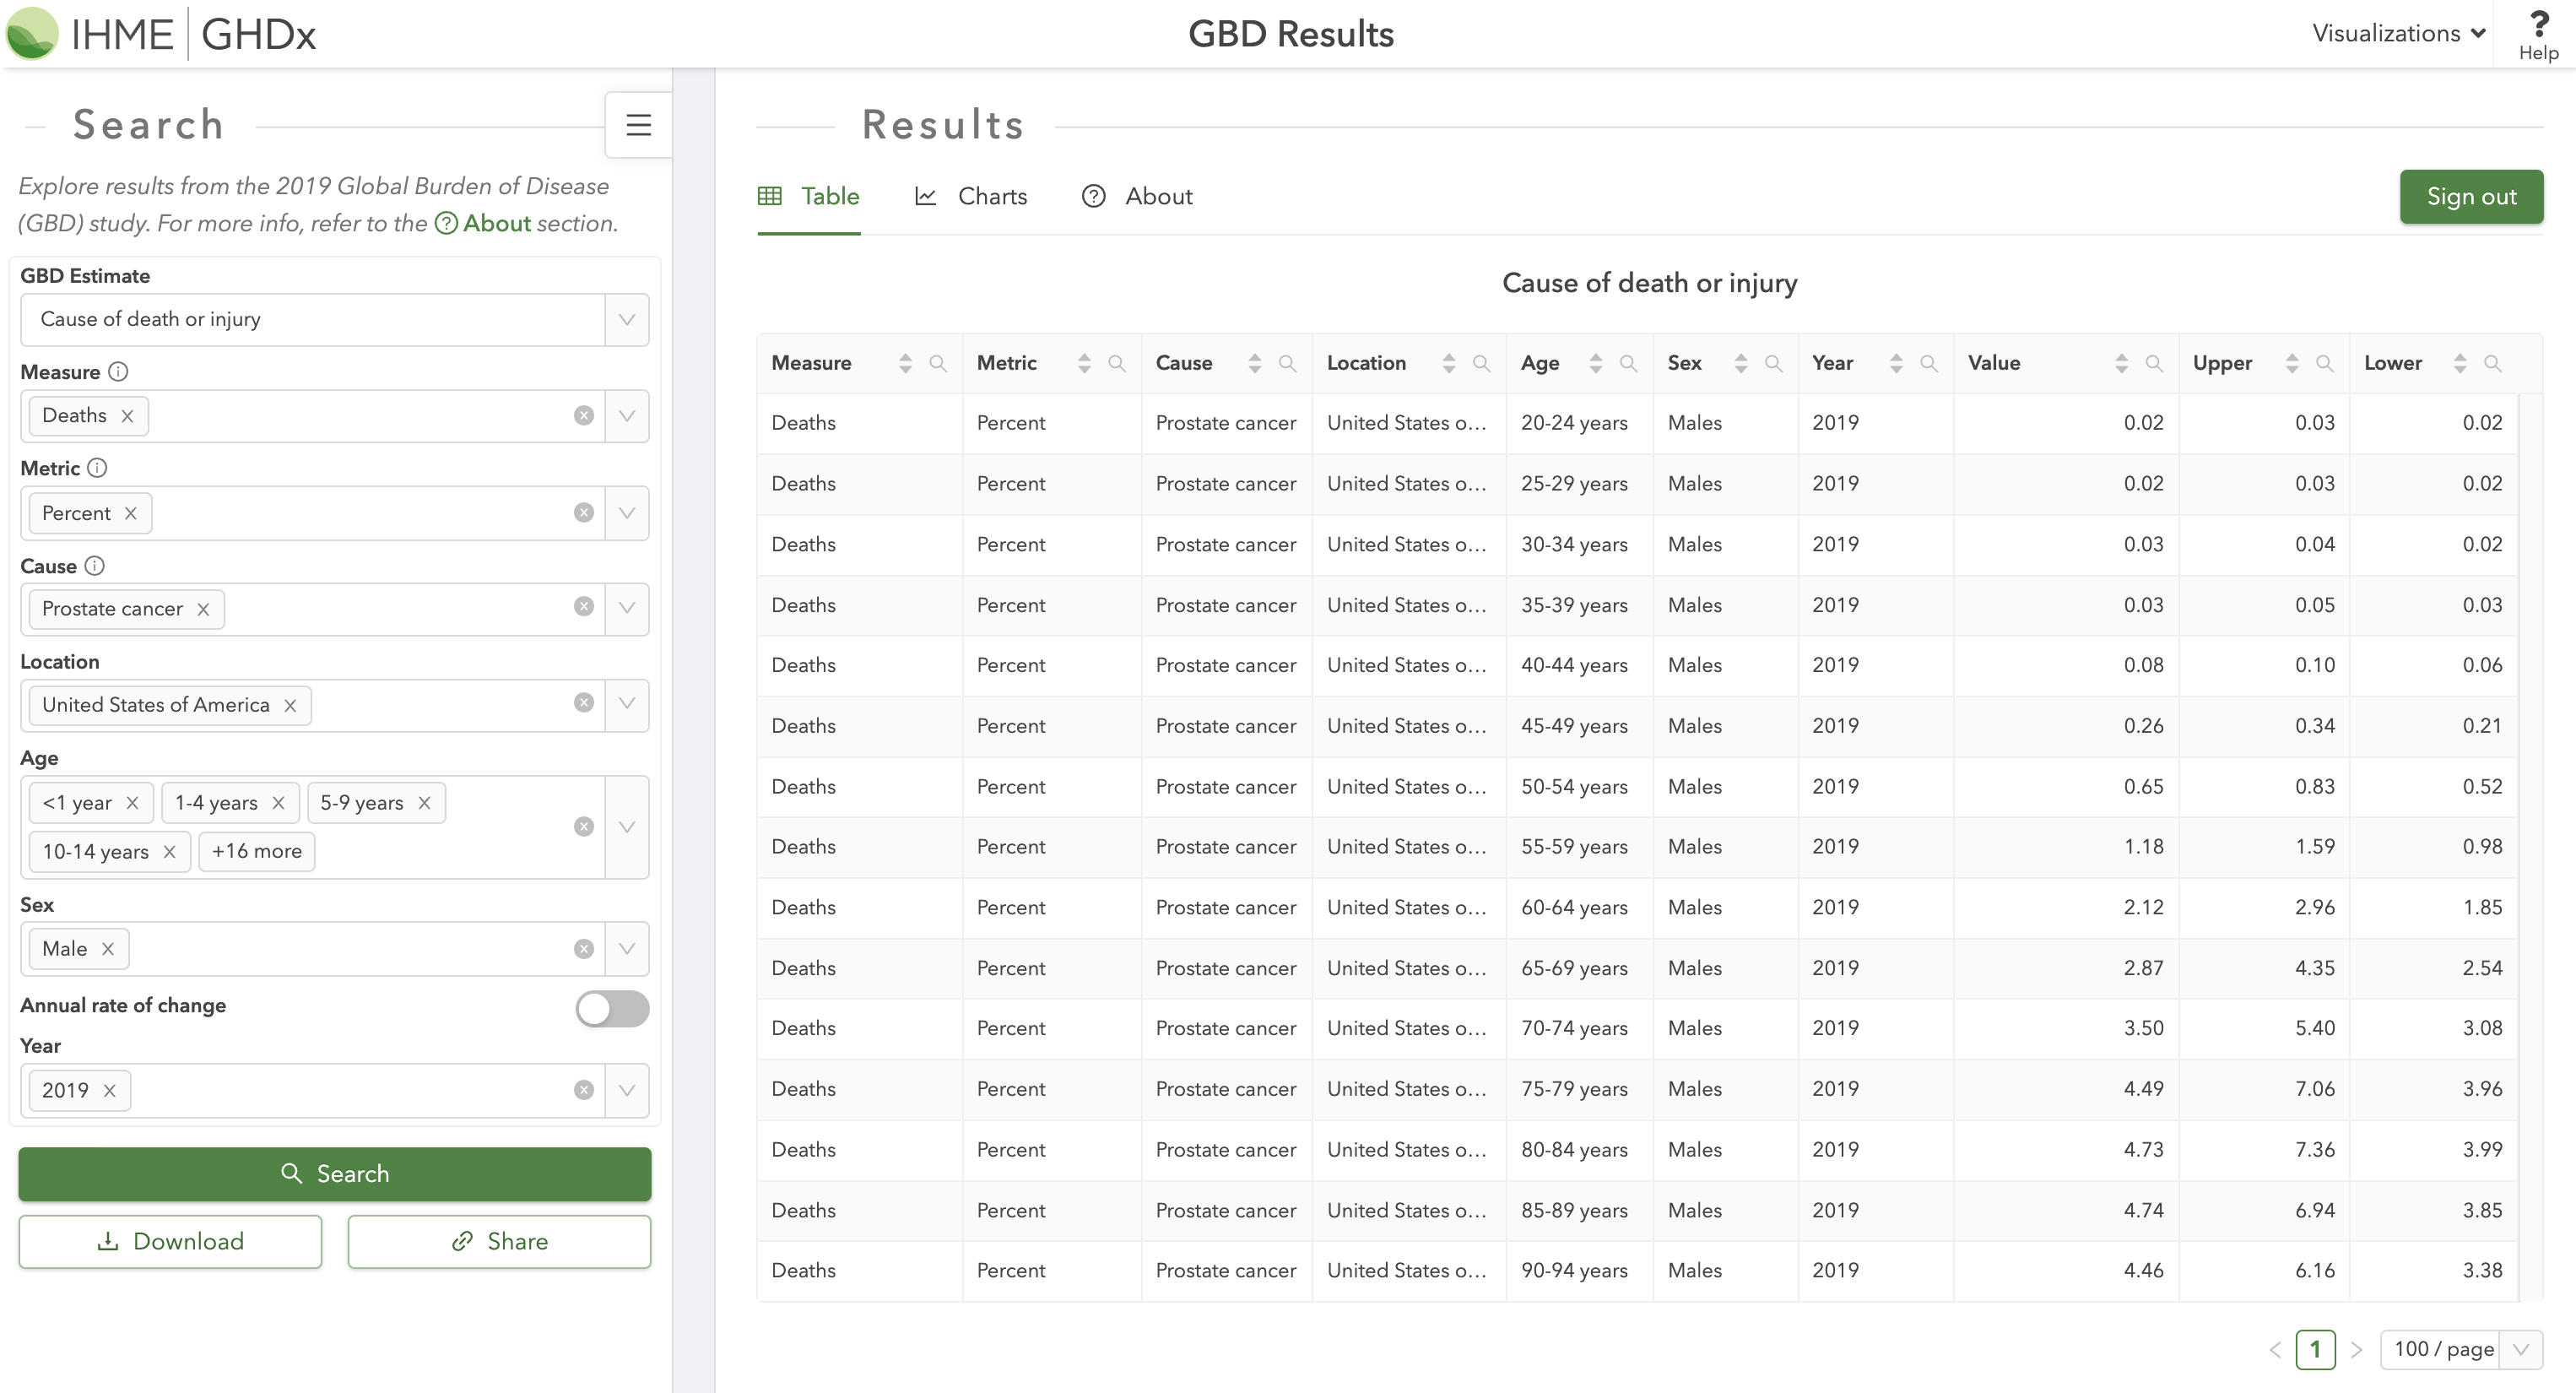
\includegraphics{exercise/prostate-cancer-cause-death.png}

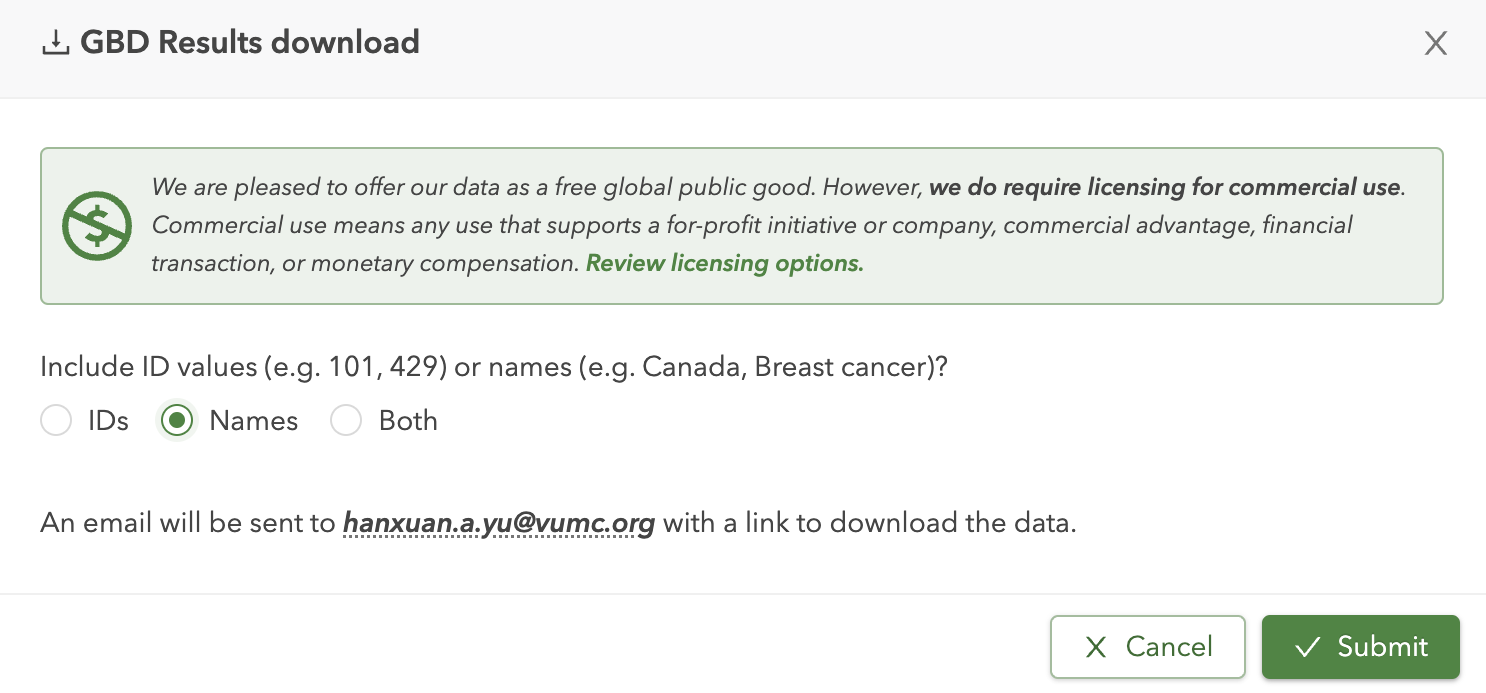
\includegraphics{exercise/GBD-download-request.png}

\hypertarget{how-to-calculate-the-cause-deleted-life-table}{%
\subsection{How to calculate the cause-deleted life
table}\label{how-to-calculate-the-cause-deleted-life-table}}

\begin{Shaded}
\begin{Highlighting}[]
\NormalTok{cause\_death\_m }\OtherTok{=} \FunctionTok{read.csv}\NormalTok{(}\StringTok{"exercise/GBD\_2019\_prostate.csv"}\NormalTok{) }\SpecialCharTok{\%\textgreater{}\%}
  \FunctionTok{select}\NormalTok{(age,val,upper,lower)}

\NormalTok{cause\_death\_m1 }\OtherTok{=}\NormalTok{ cause\_death\_m }\SpecialCharTok{\%\textgreater{}\%} \FunctionTok{filter}\NormalTok{(}\FunctionTok{str\_detect}\NormalTok{(age, }\StringTok{"\textless{}"}\NormalTok{)) }\SpecialCharTok{\%\textgreater{}\%}
  \FunctionTok{mutate}\NormalTok{(}\AttributeTok{start =} \DecValTok{0}\NormalTok{, }
         \AttributeTok{reptimes =} \FunctionTok{as.numeric}\NormalTok{(}\FunctionTok{str\_sub}\NormalTok{(age,}
                                       \FunctionTok{unlist}\NormalTok{(}\FunctionTok{gregexpr}\NormalTok{(}\StringTok{\textquotesingle{}\textless{}\textquotesingle{}}\NormalTok{, age))[}\DecValTok{1}\NormalTok{]}\SpecialCharTok{+}\DecValTok{1}\NormalTok{,}
                                       \FunctionTok{unlist}\NormalTok{(}\FunctionTok{gregexpr}\NormalTok{(}\StringTok{\textquotesingle{} \textquotesingle{}}\NormalTok{, age))[}\DecValTok{1}\NormalTok{]}\SpecialCharTok{{-}}\DecValTok{1}\NormalTok{)),}
         \AttributeTok{end =}\NormalTok{ start }\SpecialCharTok{+}\NormalTok{ reptimes }\SpecialCharTok{{-}} \DecValTok{1}\NormalTok{)}

\NormalTok{cause\_death\_m2 }\OtherTok{=}\NormalTok{ cause\_death\_m }\SpecialCharTok{\%\textgreater{}\%} 
  \FunctionTok{filter}\NormalTok{(}\FunctionTok{str\_detect}\NormalTok{(age,}\StringTok{"{-}"}\NormalTok{) }\SpecialCharTok{\&} \SpecialCharTok{!}\FunctionTok{str\_detect}\NormalTok{(age, }\StringTok{" "}\NormalTok{)) }\SpecialCharTok{\%\textgreater{}\%}
\NormalTok{  rowwise }\SpecialCharTok{\%\textgreater{}\%}
  \FunctionTok{mutate}\NormalTok{(}\AttributeTok{start =} \FunctionTok{as.numeric}\NormalTok{(}\FunctionTok{str\_sub}\NormalTok{(age,}\DecValTok{1}\NormalTok{,}\FunctionTok{unlist}\NormalTok{(}\FunctionTok{gregexpr}\NormalTok{(}\StringTok{\textquotesingle{}{-}\textquotesingle{}}\NormalTok{, age))[}\DecValTok{1}\NormalTok{]}\SpecialCharTok{{-}}\DecValTok{1}\NormalTok{)),}
         \AttributeTok{end =} \FunctionTok{as.numeric}\NormalTok{(}\FunctionTok{str\_sub}\NormalTok{(age,}\FunctionTok{unlist}\NormalTok{(}\FunctionTok{gregexpr}\NormalTok{(}\StringTok{\textquotesingle{}{-}\textquotesingle{}}\NormalTok{, age))[}\DecValTok{1}\NormalTok{]}\SpecialCharTok{+}\DecValTok{1}\NormalTok{,}\FunctionTok{str\_length}\NormalTok{(age))),}
         \AttributeTok{reptimes =}\NormalTok{ end }\SpecialCharTok{{-}}\NormalTok{ start }\SpecialCharTok{+} \DecValTok{1}\NormalTok{)}

\NormalTok{cause\_death\_m3 }\OtherTok{=}\NormalTok{ cause\_death\_m }\SpecialCharTok{\%\textgreater{}\%} \FunctionTok{filter}\NormalTok{(}\FunctionTok{str\_detect}\NormalTok{(age,}\StringTok{"{-}"}\NormalTok{) }\SpecialCharTok{\&} \FunctionTok{str\_detect}\NormalTok{(age, }\StringTok{" "}\NormalTok{)) }\SpecialCharTok{\%\textgreater{}\%}
\NormalTok{  rowwise }\SpecialCharTok{\%\textgreater{}\%}
  \FunctionTok{mutate}\NormalTok{(}\AttributeTok{start =} \FunctionTok{as.numeric}\NormalTok{(}\FunctionTok{str\_sub}\NormalTok{(age,}\DecValTok{1}\NormalTok{,}\FunctionTok{unlist}\NormalTok{(}\FunctionTok{gregexpr}\NormalTok{(}\StringTok{\textquotesingle{}{-}\textquotesingle{}}\NormalTok{, age))[}\DecValTok{1}\NormalTok{]}\SpecialCharTok{{-}}\DecValTok{1}\NormalTok{)),}
         \AttributeTok{end =} \FunctionTok{as.numeric}\NormalTok{(}\FunctionTok{str\_sub}\NormalTok{(age,}\FunctionTok{unlist}\NormalTok{(}\FunctionTok{gregexpr}\NormalTok{(}\StringTok{\textquotesingle{}{-}\textquotesingle{}}\NormalTok{, age))[}\DecValTok{1}\NormalTok{]}\SpecialCharTok{+}\DecValTok{1}\NormalTok{,}\FunctionTok{unlist}\NormalTok{(}\FunctionTok{gregexpr}\NormalTok{(}\StringTok{\textquotesingle{} \textquotesingle{}}\NormalTok{, age))[}\DecValTok{1}\NormalTok{]}\SpecialCharTok{{-}}\DecValTok{1}\NormalTok{)),}
         \AttributeTok{reptimes =}\NormalTok{ end }\SpecialCharTok{{-}}\NormalTok{ start }\SpecialCharTok{+} \DecValTok{1}\NormalTok{)}

\NormalTok{cause\_death\_male }\OtherTok{=} \FunctionTok{rbind}\NormalTok{(}
  \FunctionTok{as.data.frame}\NormalTok{(}\FunctionTok{lapply}\NormalTok{(cause\_death\_m1, rep, cause\_death\_m1}\SpecialCharTok{$}\NormalTok{reptimes)) }\SpecialCharTok{\%\textgreater{}\%}
    \FunctionTok{group\_by}\NormalTok{(age) }\SpecialCharTok{\%\textgreater{}\%}
    \FunctionTok{mutate}\NormalTok{(}\AttributeTok{Age =}\NormalTok{ start }\SpecialCharTok{{-}} \DecValTok{1} \SpecialCharTok{+} \DecValTok{1}\SpecialCharTok{:}\FunctionTok{n}\NormalTok{()) }\SpecialCharTok{\%\textgreater{}\%}
    \FunctionTok{ungroup}\NormalTok{(),}
  \FunctionTok{as.data.frame}\NormalTok{(}\FunctionTok{lapply}\NormalTok{(cause\_death\_m2, rep, cause\_death\_m2}\SpecialCharTok{$}\NormalTok{reptimes)) }\SpecialCharTok{\%\textgreater{}\%}
    \FunctionTok{group\_by}\NormalTok{(age) }\SpecialCharTok{\%\textgreater{}\%}
    \FunctionTok{mutate}\NormalTok{(}\AttributeTok{Age =}\NormalTok{ start }\SpecialCharTok{{-}} \DecValTok{1} \SpecialCharTok{+} \DecValTok{1}\SpecialCharTok{:}\FunctionTok{n}\NormalTok{()) }\SpecialCharTok{\%\textgreater{}\%}
    \FunctionTok{ungroup}\NormalTok{(),}
  \FunctionTok{as.data.frame}\NormalTok{(}\FunctionTok{lapply}\NormalTok{(cause\_death\_m3, rep, cause\_death\_m3}\SpecialCharTok{$}\NormalTok{reptimes)) }\SpecialCharTok{\%\textgreater{}\%}
    \FunctionTok{group\_by}\NormalTok{(age) }\SpecialCharTok{\%\textgreater{}\%}
    \FunctionTok{mutate}\NormalTok{(}\AttributeTok{Age =}\NormalTok{ start }\SpecialCharTok{{-}} \DecValTok{1} \SpecialCharTok{+} \DecValTok{1}\SpecialCharTok{:}\FunctionTok{n}\NormalTok{()) }\SpecialCharTok{\%\textgreater{}\%}
    \FunctionTok{ungroup}\NormalTok{()) }\SpecialCharTok{\%\textgreater{}\%}
  \FunctionTok{arrange}\NormalTok{(Age) }\SpecialCharTok{\%\textgreater{}\%}
  \FunctionTok{select}\NormalTok{(Age, val, upper, lower)}

\NormalTok{maxage }\OtherTok{=} \FunctionTok{min}\NormalTok{(}\FunctionTok{max}\NormalTok{(life\_table\_raw}\SpecialCharTok{$}\NormalTok{Age), }\FunctionTok{max}\NormalTok{(cause\_death\_male}\SpecialCharTok{$}\NormalTok{Age))}
\NormalTok{minage\_cause }\OtherTok{=} \FunctionTok{min}\NormalTok{(cause\_death\_male}\SpecialCharTok{$}\NormalTok{Age)}
\NormalTok{mlt2020 }\OtherTok{=}\NormalTok{ life\_table\_raw[(minage\_cause}\SpecialCharTok{+}\DecValTok{1}\NormalTok{)}\SpecialCharTok{:}\NormalTok{(maxage}\SpecialCharTok{+}\DecValTok{1}\NormalTok{),]}

\DocumentationTok{\#\# dx}
\NormalTok{mlt2020\_nonCause }\OtherTok{=} \FunctionTok{rbind}\NormalTok{(life\_table\_raw[}\DecValTok{1}\SpecialCharTok{:}\NormalTok{minage\_cause, }\FunctionTok{c}\NormalTok{(}\StringTok{"Age"}\NormalTok{,}\StringTok{"dx"}\NormalTok{)],}
                         \FunctionTok{data.frame}\NormalTok{(}\AttributeTok{Age =}\NormalTok{ minage\_cause}\SpecialCharTok{:}\NormalTok{maxage, }
                                    \AttributeTok{dx =}\NormalTok{ mlt2020[, }\StringTok{"dx"}\NormalTok{] }\SpecialCharTok{*}\NormalTok{ (}\DecValTok{1}\SpecialCharTok{{-}}\NormalTok{cause\_death\_male[, }\StringTok{"val"}\NormalTok{])),}
\NormalTok{                         life\_table\_raw[(maxage}\SpecialCharTok{+}\DecValTok{2}\NormalTok{)}\SpecialCharTok{:}\FunctionTok{nrow}\NormalTok{(life\_table\_raw),}\FunctionTok{c}\NormalTok{(}\StringTok{"Age"}\NormalTok{,}\StringTok{"dx"}\NormalTok{)])}

\NormalTok{mlt2020\_cause }\OtherTok{=} \FunctionTok{data.frame}\NormalTok{(}\AttributeTok{Age =}\NormalTok{ minage\_cause}\SpecialCharTok{:}\NormalTok{maxage,}
                         \AttributeTok{dx =}\NormalTok{ mlt2020[, }\StringTok{"dx"}\NormalTok{] }\SpecialCharTok{*}\NormalTok{ cause\_death\_male[, }\StringTok{"val"}\NormalTok{])}

\CommentTok{\# sum(mlt2020\_cause$dx) + sum(mlt2020\_nonCause$dx)}

\CommentTok{\# back dx to qx}
\ControlFlowTok{for}\NormalTok{ (i }\ControlFlowTok{in} \DecValTok{1}\SpecialCharTok{:}\FunctionTok{nrow}\NormalTok{(mlt2020\_nonCause))\{}
\NormalTok{  mlt2020\_nonCause[i, }\StringTok{"qx"}\NormalTok{] }\OtherTok{=}\NormalTok{ mlt2020\_nonCause[i, }\StringTok{"dx"}\NormalTok{] }\SpecialCharTok{/} \FunctionTok{sum}\NormalTok{(mlt2020\_nonCause[i}\SpecialCharTok{:}\FunctionTok{nrow}\NormalTok{(mlt2020\_nonCause), }\StringTok{"dx"}\NormalTok{])}
\NormalTok{\}}
\end{Highlighting}
\end{Shaded}

\hypertarget{build-a-loop-to-process-markov-model-background-mortality}{%
\section{Build a loop to process Markov Model \& Background
Mortality}\label{build-a-loop-to-process-markov-model-background-mortality}}

\begin{Shaded}
\begin{Highlighting}[]
\CommentTok{\# here use the cause{-}deleted life table}
\NormalTok{m\_M\_phd }\OtherTok{=}\NormalTok{ death\_background }\OtherTok{=}\NormalTok{ death\_cancer }\OtherTok{=} \FunctionTok{list}\NormalTok{()}
\CommentTok{\# setting}
\NormalTok{start\_age }\OtherTok{=} \DecValTok{45}

\ControlFlowTok{for}\NormalTok{ (i }\ControlFlowTok{in} \DecValTok{1}\SpecialCharTok{:}\NormalTok{n\_strategies) \{}
  \CommentTok{\#initialization}
\NormalTok{  death\_cancer[[v\_names\_str[i]]] }\OtherTok{=} \FunctionTok{c}\NormalTok{(}\DecValTok{0}\NormalTok{)}
\NormalTok{  death\_background[[v\_names\_str[i]]] }\OtherTok{=} \FunctionTok{c}\NormalTok{(}\DecValTok{0}\NormalTok{)}
  
\NormalTok{  m\_M\_phd[[v\_names\_str[i]]] }\OtherTok{=} \FunctionTok{matrix}\NormalTok{(}\DecValTok{0}\NormalTok{, }\AttributeTok{nrow =}\NormalTok{ params\_sc}\SpecialCharTok{$}\NormalTok{n\_cycles}\SpecialCharTok{+}\DecValTok{1}\NormalTok{, }\AttributeTok{ncol =}\NormalTok{ v\_n\_states, }\AttributeTok{dimnames =} \FunctionTok{list}\NormalTok{(}\ConstantTok{NULL}\NormalTok{, v\_names\_states))}
\NormalTok{  m\_M\_phd[[v\_names\_str[i]]][}\DecValTok{1}\NormalTok{,] }\OtherTok{=} \FunctionTok{c}\NormalTok{(params\_sc}\SpecialCharTok{$}\NormalTok{nPop, }\FunctionTok{rep}\NormalTok{(}\DecValTok{0}\NormalTok{,}\AttributeTok{times=}\DecValTok{5}\NormalTok{))}
  
  \ControlFlowTok{for}\NormalTok{ (cycle }\ControlFlowTok{in} \DecValTok{1}\SpecialCharTok{:}\NormalTok{params\_sc}\SpecialCharTok{$}\NormalTok{n\_cycles) \{}
\NormalTok{    m\_M\_phd[[v\_names\_str[i]]][cycle}\SpecialCharTok{+}\DecValTok{1}\NormalTok{,] }\OtherTok{=}\NormalTok{ m\_M\_phd[[v\_names\_str[i]]][cycle,] }\SpecialCharTok{\%*\%}\NormalTok{ m\_P[[v\_names\_str[i]]] }\SpecialCharTok{*}\NormalTok{ (}\DecValTok{1}\SpecialCharTok{{-}}\NormalTok{mlt2020\_nonCause[(cycle }\SpecialCharTok{+}\NormalTok{ start\_age),}\StringTok{"qx"}\NormalTok{] }\SpecialCharTok{\%\textgreater{}\%} \FunctionTok{pull}\NormalTok{())}

\NormalTok{    death\_background[[v\_names\_str[i]]][cycle}\SpecialCharTok{+}\DecValTok{1}\NormalTok{] }\OtherTok{=} \FunctionTok{sum}\NormalTok{(m\_M\_phd[[v\_names\_str[i]]][cycle,}\DecValTok{1}\SpecialCharTok{:}\DecValTok{5}\NormalTok{]) }\SpecialCharTok{*}\NormalTok{ (mlt2020\_nonCause[(cycle }\SpecialCharTok{+}\NormalTok{ start\_age),}\StringTok{"qx"}\NormalTok{] }\SpecialCharTok{\%\textgreater{}\%} \FunctionTok{pull}\NormalTok{()) }\SpecialCharTok{+}\NormalTok{ death\_background[[v\_names\_str[i]]][cycle]}
    
\NormalTok{    death\_cancer[[v\_names\_str[i]]][cycle}\SpecialCharTok{+}\DecValTok{1}\NormalTok{] }\OtherTok{=} \FunctionTok{round}\NormalTok{(params\_sc}\SpecialCharTok{$}\NormalTok{nPop }\SpecialCharTok{{-}} \FunctionTok{sum}\NormalTok{(m\_M\_phd[[v\_names\_str[i]]][cycle}\SpecialCharTok{+}\DecValTok{1}\NormalTok{,}\DecValTok{1}\SpecialCharTok{:}\DecValTok{5}\NormalTok{]) }\SpecialCharTok{{-}}\NormalTok{ death\_background[[v\_names\_str[i]]][cycle}\SpecialCharTok{+}\DecValTok{1}\NormalTok{],}\DecValTok{2}\NormalTok{)}

\NormalTok{  \}}
  
\NormalTok{  m\_M\_phd[[v\_names\_str[i]]] }\OtherTok{=} \FunctionTok{cbind}\NormalTok{(m\_M\_phd[[v\_names\_str[i]]][,}\DecValTok{1}\SpecialCharTok{:}\DecValTok{5}\NormalTok{], }\FunctionTok{matrix}\NormalTok{(death\_cancer[[v\_names\_str[i]]]), }\FunctionTok{matrix}\NormalTok{(death\_background[[v\_names\_str[i]]]))}
  \FunctionTok{colnames}\NormalTok{(m\_M\_phd[[v\_names\_str[i]]])[}\DecValTok{6}\SpecialCharTok{:}\DecValTok{7}\NormalTok{] }\OtherTok{=} \FunctionTok{c}\NormalTok{(}\StringTok{"Death\_Cancer"}\NormalTok{, }\StringTok{"Death\_Background"}\NormalTok{)}
\NormalTok{  \}}
  
\NormalTok{m\_M\_phd}
\end{Highlighting}
\end{Shaded}

\begin{verbatim}
$quo
      Healthy Stage1 Stage2 Stage3 Remission Death_Cancer Death_Background
 [1,]    1000      0      0      0         0          0.0              0.0
 [2,]     916     50     20     10         0          0.0              4.4
 [3,]     839     79     36     17        16          4.5              9.0
 [4,]     768     96     47     22        41         12.1             14.0
 [5,]     703    107     56     26        68         22.0             19.2
 [6,]     643    113     63     28        95         33.5             24.7
 [7,]     588    118     68     30       121         46.1             30.5
 [8,]     537    121     71     31       145         59.4             36.7
 [9,]     490    122     74     31       166         73.1             43.2
[10,]     448    123     76     31       185         87.0             50.2
[11,]     408    124     77     31       201        101.0             57.6
[12,]     372    124     77     31       215        114.9             65.5
[13,]     339    123     78     30       227        128.6             73.8
[14,]     308    122     78     30       237        142.2             82.5
[15,]     280    121     77     29       245        155.5             91.8
[16,]     255    119     77     29       250        168.6            101.5
[17,]     231    118     76     28       254        181.3            111.6
[18,]     209    115     75     27       257        193.8            122.1
[19,]     189    113     74     27       258        205.9            133.1
[20,]     171    111     72     26       258        217.6            144.4
[21,]     155    108     71     25       257        229.0            156.0
[22,]     140    105     69     24       254        240.1            167.7
[23,]     126    102     67     23       251        250.7            179.9
[24,]     113     99     65     23       247        261.0            192.3
[25,]     102     96     63     22       242        270.9            205.1
[26,]      91     92     61     21       236        280.4            218.2
[27,]      82     89     59     20       230        289.5            231.5
[28,]      73     85     57     19       223        298.2            245.1
[29,]      65     82     54     18       215        306.6            259.1
[30,]      58     78     52     17       207        314.5            273.3
[31,]      51     74     49     16       198        322.0            288.4

$trtA
      Healthy Stage1 Stage2 Stage3 Remission Death_Cancer Death_Background
 [1,]    1000      0      0    0.0         0          0.0              0.0
 [2,]     916     50     20   10.0         0          0.0              4.4
 [3,]     839     79     36   17.0        16          4.5              9.0
 [4,]     768     95     47   22.1        42         12.1             14.0
 [5,]     703    103     54   25.6        74         22.0             19.2
 [6,]     643    105     58   27.8       107         33.5             24.7
 [7,]     588    105     61   28.9       141         45.9             30.5
 [8,]     537    103     61   29.2       174         58.8             36.7
 [9,]     490    100     60   28.9       206         71.9             43.2
[10,]     448     96     59   28.2       235         84.8             50.2
[11,]     408     91     57   27.2       261         97.4             57.7
[12,]     372     87     55   26.0       285        109.5             65.6
[13,]     339     83     53   24.7       306        121.1             73.9
[14,]     308     79     50   23.4       324        132.1             82.7
[15,]     280     75     48   22.1       340        142.5             92.1
[16,]     255     71     46   20.8       354        152.3            102.0
[17,]     231     67     44   19.6       365        161.6            112.3
[18,]     209     64     42   18.4       374        170.2            123.1
[19,]     189     60     39   17.2       381        178.3            134.4
[20,]     171     57     38   16.1       385        186.0            146.2
[21,]     155     54     36   15.1       389        193.1            158.3
[22,]     140     52     34   14.2       390        199.8            170.7
[23,]     126     49     32   13.3       390        206.0            183.6
[24,]     113     47     31   12.5       388        211.9            197.0
[25,]     102     44     29   11.7       385        217.4            210.8
[26,]      91     42     28   10.9       381        222.5            225.1
[27,]      82     40     26   10.3       375        227.3            239.8
[28,]      73     38     25    9.6       368        231.8            254.9
[29,]      65     36     24    9.0       360        236.0            270.6
[30,]      58     34     22    8.4       351        239.9            286.7
[31,]      51     32     21    7.8       340        243.5            304.1

$trtB
      Healthy Stage1 Stage2 Stage3 Remission Death_Cancer Death_Background
 [1,]    1000      0      0      0         0          0.0              0.0
 [2,]     916     50     20     10         0          0.0              4.4
 [3,]     839     79     36     17        16          4.5              9.0
 [4,]     768     96     47     22        41         12.1             14.0
 [5,]     703    106     55     26        70         22.0             19.2
 [6,]     643    112     61     28        99         33.5             24.7
 [7,]     588    115     64     29       127         46.0             30.5
 [8,]     537    117     67     30       154         59.1             36.7
 [9,]     490    117     68     30       178         72.5             43.2
[10,]     448    118     69     30       200         86.0             50.2
[11,]     408    117     69     30       219         99.4             57.6
[12,]     372    116     69     29       236        112.5             65.5
[13,]     339    115     68     28       250        125.4             73.9
[14,]     308    114     67     27       262        137.9             82.6
[15,]     280    113     66     27       272        150.1             91.9
[16,]     255    111     65     26       280        161.9            101.7
[17,]     231    109     64     25       286        173.3            111.9
[18,]     209    107     63     24       290        184.3            122.6
[19,]     189    105     61     23       293        194.9            133.7
[20,]     171    102     60     22       294        205.2            145.1
[21,]     155    100     59     21       294        215.0            156.9
[22,]     140     97     57     21       292        224.5            168.9
[23,]     126     94     55     20       290        233.6            181.4
[24,]     113     91     54     19       286        242.4            194.2
[25,]     102     89     52     18       281        250.7            207.4
[26,]      91     86     50     17       276        258.8            220.9
[27,]      82     83     48     17       270        266.4            234.7
[28,]      73     79     46     16       263        273.7            248.9
[29,]      65     76     45     15       255        280.7            263.4
[30,]      58     73     43     14       246        287.3            278.4
[31,]      51     69     41     14       237        293.5            294.3

$trtC
      Healthy Stage1 Stage2 Stage3 Remission Death_Cancer Death_Background
 [1,]    1000      0      0      0         0          0.0              0.0
 [2,]     916     50     20     10         0          0.0              4.4
 [3,]     839     79     36     17        16          4.5              9.0
 [4,]     768     95     47     22        42         12.1             14.0
 [5,]     703    104     55     26        72         22.0             19.2
 [6,]     643    109     60     28       103         33.5             24.7
 [7,]     588    110     63     29       134         46.0             30.5
 [8,]     537    110     64     30       164         59.0             36.7
 [9,]     490    109     64     30       191         72.2             43.2
[10,]     448    107     64     29       216         85.4             50.2
[11,]     408    105     63     28       239         98.4             57.7
[12,]     372    103     62     28       258        111.1             65.6
[13,]     339    101     61     27       276        123.3             73.9
[14,]     308     98     60     26       291        135.2             82.7
[15,]     280     96     58     25       303        146.5             92.0
[16,]     255     93     57     23       313        157.4            101.8
[17,]     231     90     55     22       321        167.8            112.1
[18,]     209     88     53     21       327        177.8            122.8
[19,]     189     85     52     21       332        187.3            134.0
[20,]     171     83     50     20       334        196.4            145.6
[21,]     155     80     49     19       335        205.0            157.6
[22,]     140     77     47     18       335        213.2            169.7
[23,]     126     75     45     17       333        221.1            182.4
[24,]     113     72     44     16       330        228.6            195.4
[25,]     102     70     42     15       326        235.7            208.9
[26,]      91     67     41     15       321        242.5            222.8
[27,]      82     64     39     14       315        248.9            237.0
[28,]      73     62     37     13       308        255.0            251.6
[29,]      65     59     36     13       300        260.8            266.7
[30,]      58     57     34     12       291        266.3            282.1
[31,]      51     54     32     11       281        271.4            298.7
\end{verbatim}

\hypertarget{icer-re-calculation}{%
\section{ICER re-calculation}\label{icer-re-calculation}}

\begin{Shaded}
\begin{Highlighting}[]
\NormalTok{m\_M\_simplified }\OtherTok{=} 
\NormalTok{  m\_M\_phd }\SpecialCharTok{\%\textgreater{}\%} 
  \FunctionTok{map}\NormalTok{(}\SpecialCharTok{\textasciitilde{}}\NormalTok{ \{}
    \ControlFlowTok{for}\NormalTok{ (i }\ControlFlowTok{in} \DecValTok{1}\SpecialCharTok{:}\FunctionTok{nrow}\NormalTok{(.x))\{}
\NormalTok{      .x[i,}\DecValTok{6}\NormalTok{] }\OtherTok{=}\NormalTok{ .x[i,}\StringTok{"Death\_Cancer"}\NormalTok{] }\SpecialCharTok{+}\NormalTok{ .x[i,}\StringTok{"Death\_Background"}\NormalTok{]}
\NormalTok{    \}}
\NormalTok{    .x }\OtherTok{=}\NormalTok{ .x[,}\DecValTok{1}\SpecialCharTok{:}\DecValTok{6}\NormalTok{]}
    \FunctionTok{colnames}\NormalTok{(.x)[}\DecValTok{6}\NormalTok{] }\OtherTok{=} \StringTok{"Death"}
    \FunctionTok{rownames}\NormalTok{(.x) }\OtherTok{=} \DecValTok{0}\SpecialCharTok{:}\NormalTok{(params\_sc}\SpecialCharTok{$}\NormalTok{n\_cycles)}
\NormalTok{    .x}
\NormalTok{  \}}
\NormalTok{  )}

\FunctionTok{calculate\_icers}\NormalTok{(}
  \AttributeTok{cost =} \FunctionTok{get\_ce}\NormalTok{(}\AttributeTok{l\_m\_M =}\NormalTok{ m\_M\_simplified, }\AttributeTok{payoffs =} \FunctionTok{build\_payoffs}\NormalTok{(params\_sc), params\_sc)}\SpecialCharTok{$}\NormalTok{cost,}
  \AttributeTok{effect =} \FunctionTok{get\_ce}\NormalTok{(}\AttributeTok{l\_m\_M =}\NormalTok{ m\_M\_simplified, }\AttributeTok{payoffs =} \FunctionTok{build\_payoffs}\NormalTok{(params\_sc), params\_sc)}\SpecialCharTok{$}\NormalTok{qaly,}
                           \AttributeTok{strategies =}\NormalTok{ v\_names\_str)}
\end{Highlighting}
\end{Shaded}

\begin{verbatim}
     Strategy     Cost Effect Inc_Cost Inc_Effect  ICER Status
quo       quo 25104025  13832       NA         NA    NA     ND
trtA     trtA 66356870  14348 41252844        516 79971     ND
trtB     trtB 50429119  14018       NA         NA    NA     ED
trtC     trtC 73553288  14166       NA         NA    NA      D
\end{verbatim}



\end{document}
